\section{View Maintenance Concept} 
\label{sec:view_maintenance} 

In this section, we develop techniques for maintaining the following
view types in \VMS: \texttt{SELECTION}, \texttt{PROJECTION},
\texttt{INDEX}, aggregation (i.e. \texttt{COUNT}, \texttt{SUM},
\texttt{MIN}, \texttt{MAX}, \texttt{AVG}) and join
(i.e. \texttt{INNER}, \texttt{LEFT}, \texttt{RIGHT},
\texttt{FULL}). Internally, \VMS\ provides a number of auxiliary
views, which we refer to as the \texttt{DELTA},
\texttt{PRE-AGGREGATION} and \texttt{REVERSE-JOIN} view. Finally, we
explain how these view types compose to form higher level view
constructs. 
%(e.g., composing an aggregation, a selection, and a join view.)

\subsection{Auxiliary views}
\label{subsec:auxiliary_views}

Auxiliary views are internal to \VMS\ and are not exposed to
clients. They are maintained to enable, facilitate and speed up the
correct maintenance of the other view types. Some view types could not
be maintained consistently without the additional information provided
by auxiliaries, others simply benefit from their
pre-computations. While auxiliaries introduce storage overhead, they
support modularity in view maintenance; e.g., a single relation of a
multi-table-join can be reused in different join views (that embed the
same relation). Logically, auxiliaries represent the basic elements of
view maintenance and their use amortizes as more complex views are
managed by \VMS.  Auxiliaries also speed up view maintenance
significantly, as we show in Section~\ref{sec:evaluation}.  In what 
follows, we describe each auxiliary view type.

% Not important right now. We'll fix for accepted version.
% aj - above - modularity - 
%              Looking for a better term, fine for now.



\noindent  
\textbf{Delta} -- The \texttt{DELTA} view is an auxiliary view that
tracks base table changes between successive update operations.  
\TL\ entries only contain the client operation.
They do not characterize the base record state before or after the
operation. For example, for a delete operation, the client only provides
the row key, but not the associated value to be deleted, as input.
Likewise, an update operation provides the row key and new values, but
not the old values to be modified. In fact, a \TL\ entry does not
distinguish between an insert and update operation. However, for view 
maintenance, this information is vital. This motivated us to introduce 
the \texttt{DELTA} view. It records base table entry changes, tracking 
the states between entry updates, i.e., the ``delta'' between two 
successive operations for a given row.  Views that derive, have this 
information available for their maintenance operations.

\noindent  
\textbf{Pre-Aggregation} -- The \texttt{PRE-AGGREGATION} view is an
auxiliary view that prepares for aggregation by sorting and grouping
base table rows. Subsequently, aggregation views only need to apply
their aggregation function to the pre-computed state. This majorly
benefits applications that calculate different aggregations over the
same aggregation key.
%
% aj - check next sentence - we mean to say w/o P-A, VMS would ...,
%      right???
%    - just a note: we could show this benefit experimentally;
%      not important right now
%
To materialize these aggregates without our pre-aggregation,
\VMS\ would have to fetch the same record over and over. Moreover, for
\texttt{MIN} and \texttt{MAX} views, the deletion of the minimum
(maximum) in the view would require an expensive base table scan to
determine the new minimum (maximum), introducing consistency issues
that result from the sought after value changing while a scan is in
progress, shown by the analysis in~\cite{jacobsen:viewmaintenance}.
This motivated us to introduce the \texttt{PRE-AGGREGATION} view. This
view type sorts the base table records according to the aggregation
key, storing the grouped rows in a map. Aggregation functions like
\texttt{COUNT}, \texttt{SUM}, \texttt{MIN}, \texttt{MAX} or
\texttt{AVG}, can then be applied to the map. Thus, aggregation
results become available instantaneously.

\noindent  
\textbf{Reverse Join} -- A \texttt{REVERSE-JOIN} view is an
auxiliary view that supports the efficient and correct materialization
of join views in \VMS.  A \texttt{JOIN} view is derived from at least two
base tables. For an update to one of these tables, the \VM\ needs to
query the other base table to determine the matching join rows. Only
if the join-attribute is the row key of the queried base table, can
the matching row be determined quickly, unless of course, an index is
defined on the join-attribute for the table.  Otherwise, a scan of the
entire table is required, which has the following drawbacks: (i) Scans
require a disproportional amount of time, slowing down view
maintenance. Also, with increasing table size, the problem worsens. (ii)
Scans keep nodes occupied, slowing down client requests.  (iii)
While a scan is in progress, underlying base tables may change, thus,
destroying view data consistency for derived views. To address these 
issues, we introduce the \texttt{REVERSE-JOIN} view.

We take the \textit{join key} ($jk$) of the two base tables as row key
of the \texttt{REVERSE-JOIN} view. When updates are propagated, the
\texttt{REVERSE-JOIN} view can be accessed from either side of the
relation with the help of the join key (it is always included in both
tables' updates). If a record is inserted into one of the underlying
base tables, it is stored in the \texttt{REVERSE-JOIN} --- whether or
not it has a matching row in the other base table.

This technique enables \texttt{INNER}, \texttt{LEFT}, \texttt{RIGHT},
and \texttt{FULL} joins to derive from the \texttt{REVERSE-JOIN} view
without the need for base table scans, as we show below.


\subsection{Standard views}
\label{subsec:common_views}

In this section, we describe how \VMS\ maintains client-exposed views
for a number of interesting standard view types. We also present
alternative maintenance strategies, but defer a full-fledged
analytical cost analysis to future work.

\noindent  
\textbf{Selection and Projection} -- A \texttt{SELECTION} view selects
a set of records from a base table based on a \textit{selection
  condition}. A \texttt{PROJECTION} view selects a set of columns from a base
table. Similar to the \texttt{SELECTION} view, the \VM\ uses the row
key of the base table as row key for the view table. To save storage and 
computation resources, we can combine \texttt{DELTA}, \texttt{PROJECTION} and
\texttt{SELECTION} into a single view. This would reduce the amount of
records (due to selection), the amount of columns (due to projection),
and still provide delta information to subsequent views. These
considerations are important for multi-view optimizations with \VMS,
which we defer to future work.

\noindent  
\textbf{Aggregation} -- The maintenance of \texttt{COUNT} and
\texttt{SUM} views is similar, so we treat them together.
Generally speaking, in aggregation views, records identified by an
\textit{aggregation key} aggregate into a single view table record.
The aggregation key becomes the row key of the view. 

\texttt{MIN} and \texttt{MAX} views are
also aggregates. Both can be derived from a \texttt{DELTA} or a
\texttt{PRE-AGGREGATION} view. When derived from a \texttt{DELTA}
view, \texttt{MIN} and \texttt{MAX} are computed similar to a
\texttt{SUM}. However, a special case is the deletion of a minimum
(maximum) in a \texttt{MIN} (\texttt{MAX}). In that case, the new
minimum (maximum) has to be determined. Without auxiliary views, a
table scan would have to be
performed~\cite{jacobsen:viewmaintenance}. This motivated us to derive
the \texttt{MIN} (\texttt{MAX}) from a \texttt{PRE-AGGREGATION}, which
prevents the need for a scan.

\noindent
\textbf{Index} -- \texttt{INDEX} views are important to provide fast
access to arbitrary columns of base tables. The view table uses the
chosen column as row key of the view, storing the corresponding table
row keys in the record value. If the client wishes to retrieve a base
table row by the indexed column, it accesses the \texttt{INDEX} view
first, then, it accesses the base table with the row keys retrieved
from the record found in the view. This is a fast type of access, for
the client is always accessing single rows by row key. 
%The
%\texttt{INDEX} view is a special case of the \texttt{PRE-AGGREGATION}
%view. If the indexed key is the same as the aggregation key, we can
%combine both view types. Further, the \texttt{PRE-AGGREGATION} can be
%combined with a \texttt{REVERSE-JOIN} view (see description above).
%Thus, we receive three different view types at the cost of one.

\noindent
\textbf{Join} -- A \texttt{JOIN} view constitutes the result of
joining $n$ base tables. Since the matching of join partners is
already accomplished by the associated \texttt{REVERSE-JOIN}, the
actual \texttt{JOIN} simply serves to combine the results in the
correct way.  To obtain the join result,
%
% aj - below - ``output operations'' is not clear
%              ``multiplies column families'' is not clear
%               Try to explain this more clearly.
%
the update program takes the output operations of the
\texttt{REVERSE-JOIN} and multiplies their column families. In this
manner, the \texttt{INNER}, \texttt{LEFT}, \texttt{RIGHT}, and
\texttt{FULL} join can be maintained, easily. So far, we are only 
providing equi joins. Theta joins, with more complex join predicates
are deferred to future work.

\subsection{View composition}
\label{subsec:view_chain}

\begin{figure*}
\minipage{1\textwidth}
  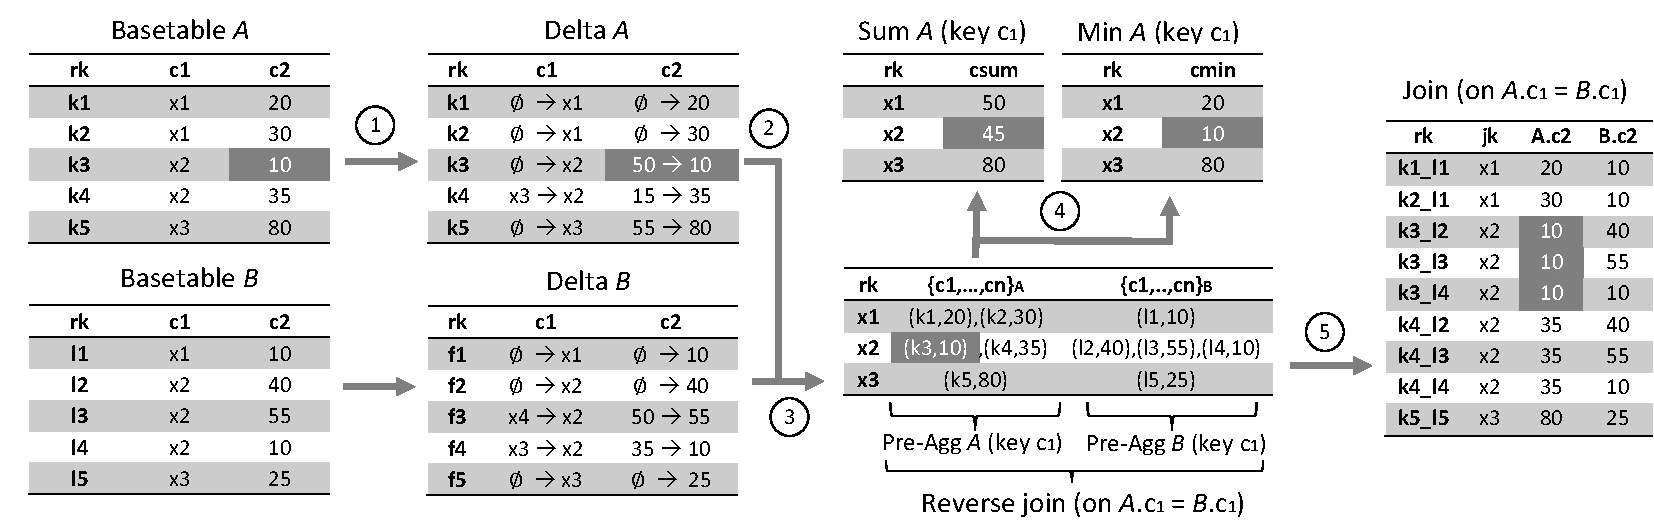
\includegraphics[width=\linewidth]{figures/ViewCalculationExample}
  \caption{View table example}\label{fig:view_table_example}
\endminipage\hfill
\vspace{-2mm}  
\end{figure*}

Figure~\ref{fig:view_table_example} gives a comprehensive example of
the introduced view types (standard and auxiliary). On the left side,
two base tables $A$ and $B$ are shown. Both base tables consist of a
row key ($rk$) and two columns ($c_1, c_2$). Either base table is
connected to a delta table (Delta $A$ and $B$) that tracks the changes
of base table columns. The delta tables are connected to a
\texttt{PRE-AGGREGATION} and a \texttt{REVERSE-JOIN}, respectively.
These views reorder and group the base table records according to a
secondary key (found in columns $A.c_1$ and $B.c_1$)\footnote{One may argue
that groups of such an aggregation tend to grow very large (if
the total number of aggregation keys is small). However, due to the
column-oriented storage format of many \KVS, the values are stored
consecutively and indexed by column key -- the access still remains
fast.}.

%
% aj - above - ``column-oriented storage format'' has not been 
%              discussed in our background, has it? Or, we may add
%              a footnote to qualify/explain a bit more.
%
In the set-up of Figure~\ref{fig:view_table_example}, aggregation key
(of \texttt{SUM} and \texttt{MIN}) and join key (of \texttt{JOIN}) are
equal, so the \texttt{PRE-AGGREGATION} becomes a subset of the
\texttt{REVERSE-JOIN}. This is a good example of how a single
auxiliary view can feed multiple different views to reduce the overall
cost. The column set ($\{\}_A$) in the \texttt{PRE-AGGREGATION} serves
to directly determine the values of \texttt{SUM} and
\texttt{MIN}. Further, the cross-product of column sets $\{\}_A$ and
$\{\}_B$ serves to maintain the \texttt{JOIN} at the right side of the
figure.

The grey arrows in Figure~\ref{fig:view_table_example} depict the
paths along which the client operations are propagated to update the
view composition.  Instead of re-computing the complete views, just
the affected parts are modified. To further reduce overhead, \VMS\ 
can execute updates on single view column values; the rest of the row 
remains unaltered. 

%
% aj - below - I have a bit diffuclty understanding the below
%              also, we speak of row / column key; I believe, this
%              has not been discussed in Background
%
\textit{Example:} Now, we show a put operation that triggers a number
of updates along the view composition (see
Figure~\ref{fig:view_table_example}, the dark grey boxes): (1) The put
operation changes the value of row $k_3$, column $c_2$ in base table
$A$ from $50$ to $10$. (2) The change is propagated and represented in
Delta $A$ as $50\rightarrow 10$. (3) The corresponding column in the
\texttt{PRE-AGGREGATION} view (i.e., row key $x_2$, column
$\{c_1\}_A$) is updated. (4) This causes the sum and minimum of row
key $x_2$ in the \texttt{SUM} and \texttt{MIN} to be re-evaluated. (5)
Further, the corresponding entries in \texttt{JOIN} are updated to the
new value $10$. As depicted, \VMS\ always accesses a single column
value (to update the view tables); the access is executed with
knowledge of row and column key. Since a \KVS\ guarantees fast row and
column key access, -- actually, this is what they are built for, --
the update propagates rapidly through the composition.  Besides the
example in Figure~\ref{fig:view_table_example}, more complex view
compositions can be created by combining different types of view
tables.

% aj - This is a bit strong. SQL is a very complex language; VMS does
%      support full fledged SQL somebody could argue
%
%... such that any kind of SQL-query can be expressed.
%








 








